
%(BEGIN_QUESTION)
% Copyright 2006, Tony R. Kuphaldt, released under the Creative Commons Attribution License (v 1.0)
% This means you may do almost anything with this work of mine, so long as you give me proper credit

Et målesystem med bånd og flottør skal brukes til å måle nivået på grenseflaten mellom olje og vann i en lagertank:

$$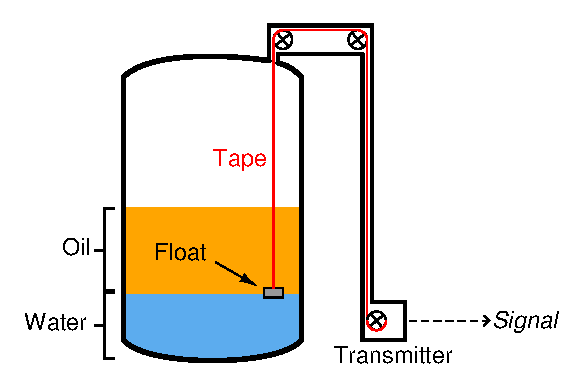
\includegraphics[width=15.5cm]{i00517x01.eps}$$

Selve flottøren må ha riktig tetthet for å flyte i vann, men synke i olje, slik at den legger seg i likevekt (nøytral oppdrift) ved grenseflaten mellom de to væskene. Oppgaven din er å lage en flottør som fungerer i denne applikasjonen.

En hul skive av tynnmetall er utgangspunktet for flottøren. Den har diameter 21 tommer og høyde 3 tommer:

$$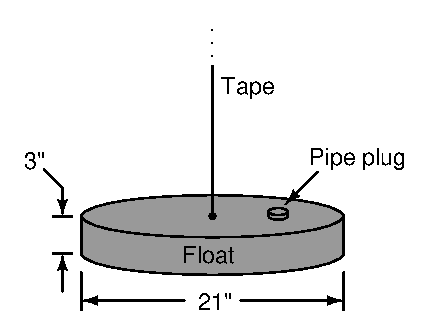
\includegraphics[width=15.5cm]{i00517x02.eps}$$

Selv om flottøren er hul, finnes en rørplugg på toppen som kan tas ut, slik at du kan fylle blyhagl (``shot'') inni flottøren for å gjøre den tyngre og dermed endre effektiv tetthet. Uten blyhagl veier flottøren 10 pund.

Beregn hvor mye blyhagl som må legges inn i flottøren for å oppnå riktig tetthet slik at den flyter i grenseflaten mellom olje og vann. Anta spesifikk vekt 0.81 for oljen.

\vskip 10pt

Mengde blyhagl som skal legges inni flottøren = \underbar{\hskip 50pt} lbs

\vskip 10pt

Merk: det finnes et {\it intervall} av korrekte svar på denne oppgaven. Du får full uttelling dersom svaret ditt ligger innenfor dette intervallet.

\underbar{file i00517}
%(END_QUESTION)





%(BEGIN_ANSWER)

Mengde blyhagl som skal legges inni flottøren = \underbar{\bf 20.4 to 27.5} lbs

\vskip 10pt

10 poeng for riktig svar, halv uttelling dersom svaret ikke inkluderer vekten av metallflottøren (-10 pounds, som gir intervallet 10.4 til 17.5 pounds haglvekt)

%(END_ANSWER)





%(BEGIN_NOTES)

{\bf Denne oppgaven er ment for eksamen, ikke arbeidsark!}.

%(END_NOTES)

